% INNAN DU COMMITAR!
% Uppdatera datum
% Uppdatera version
%-----

\documentclass[10pt,a4paper]{article}
\usepackage[utf8]{inputenc}
\usepackage[english]{babel}
\usepackage{amsmath}
\usepackage{amsfonts}
\usepackage{amssymb}
\usepackage{graphicx}
\usepackage{geometry}

\title{PostCardBuddy}
\author{Team C}

\begin{document}
\begin{titlepage}
\newgeometry{left=2cm,top=1cm,right=2cm}
\newcommand{\HRule}{\rule{\linewidth}{0.5mm}}


\begin{flushright}
December 8, 2015 v2.02\\[3cm]
\end{flushright}


\centering
\textsc{\LARGE Team C}\\[0.5cm]

\HRule \\[0.4cm]
{ \huge \bfseries PostCardBuddy}\\[0.3cm]
{\Large \bfseries Project Experiences}\\[0.4cm] % Title of your document
\HRule \\[1.5cm]

\vfill
\begin{flushleft}
%Authors, write on separate lines
\textit{Authors of this document:}\\
Emma Albertz\\
Caroline Brandberg\\
Linnéa Claesson\\
Billy Johansson\\
Johan Ju\\
Jacob Mejvik\\
Carl Rynegardh
\end{flushleft}

\end{titlepage}
\pagenumbering{gobble}



%\begin{center}
%\textit{\large Version History}
%
%    \begin{tabular}{ | l | l | l | p{5cm} |}
%    \hline
%    \textbf{Version} & \textbf{Date} & \textbf{Responsible} & \textbf{Description} \\ \hline
%    1.0 & 2015-10-14 & EA, LC & Baseline\\ \hline
%    \end{tabular}
%\end{center}



\setcounter{tocdepth}{2}
\tableofcontents
\newpage
\pagenumbering{arabic}

%---------------------------------------------------------------%
% A description of our requirements engineering work, including experiences and reflections in relation to learning objectives.
% The Project Experiences should not include course evaluation issues, but focus on your own work and learning outcome.
%---------------------------------------------------------------%

%-------------------------------------------------------------------%
%-------------- Background -----------------------------------------%
%-------------------------------------------------------------------%
\section{Introduction}
This document aims to describe how the work has been conducted during the project. It also contains the group's reflections on the work process and the difficulties with different parts of the project. 


%-------------------------------------------------------------------%
%--------------- Methods and Techniques ----------------------------%
%-------------------------------------------------------------------%
% Description of the chosen methods/techniques for elicitation, specification, validation, and prioritization.
% Motivation for why you chose the used methods/techniques.
\section{Methods and Techniques}
\label{sec:mat}
A description of the methods and techniques will be presented in this section, along with a short motivation for why the specific technique was chosen. In section~\ref{sec:ref} can evaluations of the used methods and techniques be found.

% 3D) apply more than one elicitation technique in a relevant way.
\subsection{Elicitation}
To find relevant elicitation techniques, \textit{Software Requirements - Styles and Techniques} by Soren Lauesen has been used as a guidance\cite{soren}.

The initial identification of relevant stakeholders emanated from a discussion about the product and who interacts with it. From this discussion the stakeholders that were the most important for this product could be identified. Since it was important to quickly get going with the project this method was considered appropriate. The group is well aware that this approach could cause important stakeholders to be left out. In order to reduce this risk, identification of other stakeholders have been a top priority through out the project. The product is somewhat limited in scope and hence the number of additional stakeholders that have been considered significant have been few. 

The following elicitation techniques were used:
\begin{description}
\item[Brainstorming] Used as a first step within the team to come up with basic ideas and functions of the product. This is a quick method to get some initial ideas and starting points. During the brainstorming session the functions specified by the key customer, from their initial order of the product, were also considered.

\item[Questionnaire] The questionnaire was sent out to people within the end user group. Questions from the brainstorming session were used to form the questions. People answering were asked to grade functions from zero to five, where zero stood for not interesting and five for very interesting. An age field was added to see if there was a difference in interest of various functions between ages. This is also an easy method to get some ideas of what the intended users of the product might want (or not want).

\item[Interviews] In order to improve the understanding of the kind of product envisioned by the key customer, an interview session was conducted early in the elicitation process. 

\item[Prototypes] Three team members created one prototype each, independently of each other so as not to affect each other's ideas. It was decided to do this right away due to the time constraint upon this project. The prototypes are meant to be used for ideas to the graphical interface of the application. The use of prototypes is considered a suitable technique for this project since there are many easy to use and free programs available to create them. Additionally, it gives not only the stakeholders but also the authors of the requirements a good idea of what it should look like and be able to do. They were specifically used when eliciting requirements from prospective end users.

\item[Document study] There is already a similar existing application on the market and it was used to further elicit functionality not already thought of and also to perhaps eliminate functionality that intervenes with the user experience. This was done \textit{after} the initial brainstorming session, to avoid making an identical application or interfere with the creativity of the team. 

\item[Data model]

\item[Data dictionary/Virtual windows]

\item[Summary] In the elicitation process several different elicitation techniques were used. The group has continuously reflected on the choices and experiences from the various techniques. In some cases the reflections has highlighted the need for more information, resulting in that additional elicitation has been conducted. However, there are still some areas that require further elicitation as the development of the product commences. As an example, a specific area that deliberately has been kept somewhat limited is the exact technical specifications. 
The elicitation process has also been heavily geared towards going beyond the initial stakeholders and challenge the domain borders. In doing so, several potential stakeholders, such as traveling companies and advertisement agencies, have been considered. The stakeholders that have been left out of the final project has been deemed to have little relevance to current structure of the project. In some cases, e.g traveling agencies, potential stakeholders could have been attributed with a higher relevance given a different business model for the product. Furthermore, in order to broaden and deepen the understanding of the domain stakeholders have been contacted. Although, this has given valuable feedback in most cases it also underlined some difficulties. For example, when contacting the postal services it proved difficult to get in touch with relevant staff to answer our rather technical questions. 

\end{description}


% 4B) use at least four different specification techniques adequately tailored to the context.
\subsection{Specification}

\begin{description}
\item[Context diagram] A context diagram was used since it is easy to make and is helpful when time comes for validation and verification. The diagram gives a good over-view of the system, both for the use of the client but also for the developers. 

\item[Data model]

\item[Data dictionary/Virtual windows]

\item[Quality grid]
A quality grid was created by brainstorming what quality aspects was important for PostCardBuddy. This was done by starting out from Lauesens quality grid on page 227 \ref{bibitem:soren}. Lauesen's quality grid was stripped down to the parts, we thought, was worth mentioning. Doing the strip down, a few questions guided us:
\begin{description}
\item What quality aspects are more important for PostCardBuddy in comparison to other applications/software.
\item Is their something we would like to describe more to the developers.
\item How do we rank each of the quality factors.
\item How do we set the quality factors and their ranking into context. Meaning, how do explain why this is important to the developers.
\end{description}

Many "As usual" quality factors where left out because we thought that there was no use to explain them.

\item[QUPER]
A Quper diagram was created to specify a Quality requirement, or perhaps target is a better word. Quper is documented in ref LÄGG IN. Document studies of the competitor "Riktiga Vykort" showed that requesting images from their image library into creating a postcard was a painful process. If PostCardBuddy could be better in this aspect it would be highly valuable. Quper as in ref !!!! contains advanced features requiring a lot of knowledge in the domain. Not having this knowledge, a lot parts where left out so just the basics were left. To get a feel for what would be a reasonable target, in case of user experience, testing was done with "Riktiga Vykort". As we did not have enough knowledge for the technical aspect this was, more or less, left out.

\end{description}

% 3F) to assess the quality of requirements and find relevant problems of several different types.
% 3G) apply more than one validation technique.
% 4G) adapt the validation to the context and provide rationale for the chosen validation techniques.
\subsection{Validation}
\begin{description}
\item[Prototypes] The prototype gives the customer a unique opportunity to validate how the product matches their expectations. The prototypes will be continuously adapted to the customer's needs and wants and new features will be added (or others removed) so that it becomes a good reflection on where the project is going. 

\item[Validation checklists and validation report (as developers)]

\item[Validation checklists and validation report (as customers)] Validation checklists provided by the developer group were used to validate the product initially ordered as customers. A validation report was then written based on the checklists.

\item[Informal review]
\end{description}


% 3I) use more than one prioritization technique in a relevant way.
\subsection{Prioritization}
\begin{description}
\item[Stakeholders] The prioritization for each stakeholder was stated through discussions within the group.  
\end{description}
%--------------------------------------------------------------------%
%--------------- Reflections ----------------------------------------%
%--------------------------------------------------------------------%
% Reflection on the usage of these methods/techniques in terms of what was successful and what was challenging. Example questions for reflection: What have you learned in relation to the learning objectives in this course program? What would you have done differently if you would do this project again as a "real" project, based on what you know now? What have you learned in relation to the learning objectives?


% Osäker om detta är rätt placering: 5B) provide motivated estimations of target quality levels using well-defined scales.
% 4F) to find, prioritize and discuss requirements quality problems of different types, while reaching 	beyond form issues.
% 5D) reason about the relation between requirements quality problems and risks, both from a customer and developer viewpoint.
\section{Reflections}
\label{sec:ref}

% 3E) reflect on elicitation experiences.
% 4E) reason about the need for further elicitation in relation to specification quality.
% 5C) go beyond initial stakeholders and given frames, while challenging the domain boundaries and eliciting creative ideas and deep domain knowledge in real-world contexts.
This section aims to evaluate the methods and techniques used, as described in section~\ref{sec:mat}
\subsection{Elicitation}
\begin{description}
\item[Brainstorming]The reason for selecting the method to collect our stakeholders was because it is a fast method which meant that is was possible to start working, such as contact some of the stakeholders. 

\item[Questionnaire] Figure~\ref{fig:questionnaire} presents the result of the questionnaire, which 38 people answered. To get answers from that amount of people was no problem and it gave a first idea of what the users were interested in. The result of this is that the functionality "Share postcard on social media" was not important and "Suggestion for GPS-based images" was appreciated. The result also showed that the desired functionality did not change that much depending on the age. Using a questionnaire was interesting since it gave a good idea of the functions people are interested in. However, as the questionnaire  was created it was desirable that it was quick to answer. Therefore, only ten questions were used to maximize the number of respondents and the quality of the replies. Afterwards it was realized that some interesting functionalities were missing. Knowing the interest of these functionalities as well could have been of interest and might be investigated further prior future releases.

\item[Interviews] Although the interview provided valuable insights the main impression was ambiguity, both in terms of the role the key customer would have and exactly what the product should do. Given more time it would have been beneficial to invest in achieving a better consensus within the customer group before conducting the interview. Additional interviews will be conducted during the requirements specification process.

Furthermore, two separate companies in the postal service business have been contacted with the intention to conduct interviews. However, it has proved difficult to get past the first line support and get a hold of an appropriate contact. A possible explanation for this is that the postcard business is only a minor part of the postal services market and there is probably nobody with a clear responsibility for this area.  

\item[Prototypes] A program was used for constructing the prototypes that worked very well. It also proved to be of use for brainstorming new ideas and features, since the program itself offered a lot different options on how to do things. 

From discussions with the costumer team, new ideas for features emerged when the costumer tried the prototypes. The prototype helped the costumer to verify that the application conformed to their requirements and also gave them an opportunity to see if something was missing or wrong.

\item[Document study] The already existing application is easy to use and slim. It does not contain a lot of functions but there are enough. Most of the basic functions are already implemented. However, there are definitely some functionalities that could be of use that are not implemented. Also, the library of images is not very big and GPS based images depending on your localization only works in Sweden and Denmark. All of the above was helpful.

\item[Data model] Creating the data model for the data requirements was in itself an exercise in elicitation. While gradually developing the ER-diagram new entities and relationships that were not easy to spot in the beginning started to emerge. This was largely due to dependencies between between different types of required data.

\item[Data dictionary/Virtual windows] Creating a data dictionary or virtual windows is a lot similar to doing a data model, from an elicitation point of view. Doing all three might be unnecessary (if elicitation is the purpose), but doing two of them would definitely be of value. The virtual windows technique especially is good for realizing what types of data might be missing from a certain feature.
\end{description}


\begin{figure}[h!]
\centering
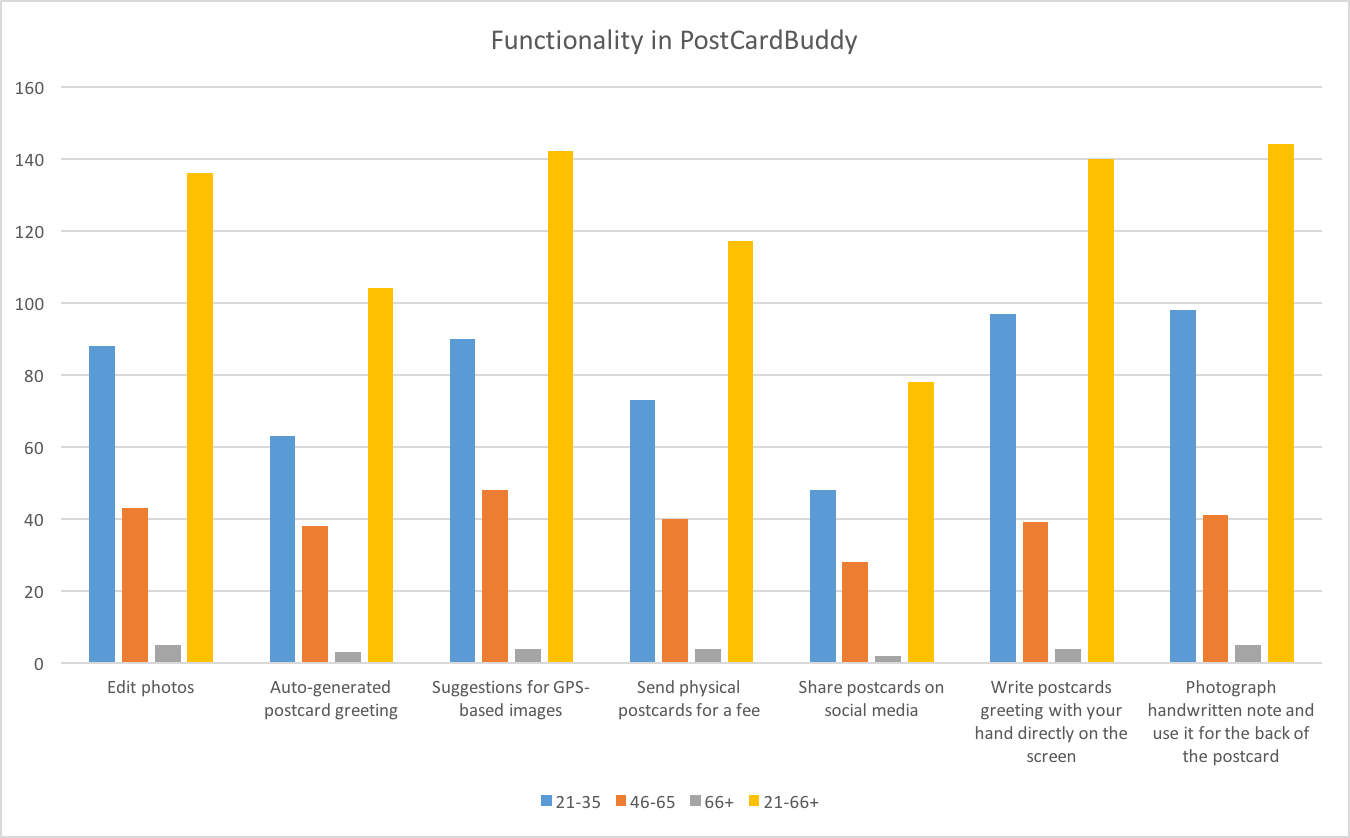
\includegraphics[width=1.0\textwidth]{questionnaire.png}
\caption{Result of the questionnaire on the desired functionality in PostCardBuddy}
\label{fig:questionnaire}
\end{figure}
% Ska vi �ven ha en figur som presenterar hur m�nga 0,1,..5 varje funktion fick???


% 3C) reflect on specification experiences and reason about choices of specification methods in relation to different contexts.
% 5A) combine specification techniques in an explicitly motivated trade off between qualities and costs, where a high degree of specification completeness is achieved for a carefully selected subset of requirements.
\subsection{Specification}
\begin{description}
\item[Context diagram] The first context diagram created was presented in PMv2. The first diagram was very limited and contained too little information to understand the system. The updated diagram was then presented in release 1 of the report System Requirements. The biggest problem creating a context diagram was that it should be big enough to present important details, but small enough to be able to get an overview of the system. Therefore it is very important to think through which components it should contain, and which should be left out. This difference is often personal, which was noticed during the creation of release 1, which led to some discussion. Most of the discussion were spent talking about if the back-end should be presented and how the functionality that is used within the mobile should be presented. 

The changes of the context diagram between release 1 and release 2 were mostly added descriptions of the parts. These descriptions were easily added without any problem. Also the contacts were added, which was a part that was missing in the previous version. It is very easy to miss parts of the diagram. To find out that every part is within, it is very good to try to describe each chain and see if it is easy from that description to follow in the context diagram. 

\item[Data model] The data model is a good tool to easily visualize dependencies of different systems and stakeholders. If done  thoroughly it could be used as a good starting point for developers, and in particular database developers. But the more complicated the data model becomes, the harder it gets for non-technical personnel to understand it. And in the same way it loses some of its value for developers if it is not thorough enough. This is why it was combined with  a data dictionary and virtual windows, to adequately satisfy technical as well as non-technical personnel. 

\item[Data dictionary/Virtual windows] The data dictionary is probably the simplest tool for specifications. It is easy to write but can become tedious and it is hard to see relationships between data. As a complement to a data model it is very good for properly communicating a specification. Virtual windows are very helpful for non-technical personnel and is a very efficient way of presenting an overview of what types of data are needed for a specific feature. 

\item[Quality grid]
Doing a quality grid was a very good idea. While creating the quality grid many ideas came to life. Especially ideas for different requirements.
The quality grid should probably have been created early in the project phase. Maybe even in the first week together with stakeholders. While creating the quality grid you get forced to think of different aspects of the application. You get some kind of overview over what is important, and with that ideas come to life. Therefore, a quality grid could be a way of elicitating, mostly quality factors, but maybe even functional requirements. The line between quality requirements and functional requirements can be very thin. A negative aspect with the Quality grid is that it does not have any requirements. It mostly highlights what is important for the application and describes to the developer why this is important. If it really is a negative aspect could be discussed, as it is a very useful way of communicating quality factors to the developers. As the Quality grid was created rather late in the project, we did not base any quality requirements on it. If the quality grid would have been created early, quality requirements could also been based on the grid. This would have complimented the Quality grid.


\item[QUPER]
It is interesting to compare the quality grid with Quper. The quality grid gives a better overview over quality factors as a whole while Quper serves as a way to specify a target or requirement. Normally, Quper demands a lot of knowledge which we did not have. Therefore, it was not very useful in our case. It did highlight the problem with the competitor "Riktiga Vykort"'s application and specified how long time it should take for PostCardBuddy, but this could have been done in different ways. If we would have more knowledge in the domain Quper would probably have been more useful.


\end{description}




% 3H) reflect on validation experiences.
% 5E) utilize links among different types of specifications in validation efforts to find and address potentially harmful inconsistencies.
\subsection{Validation}
\begin{description}
\item[Prototypes]

\item[Validation checklists and validation report (as developers)]


\item[Validation check lists and validation report (as customers)] The use of checklists was very helpful as it is easy to check the quality of existing requirements. However, it is also limiting in the sense that it makes it difficult to see if there are any missing requirements. It is easy to "get stuck inside the box" that the checklist actually is. Checklists are very quantitative and need explaining comments in addition to get qualitative information from them.

\item[Informal review]


\end{description}

% 3J) reflect on prioritization experiences.
\subsection{Prioritization}
\begin{description}
\item[Stakeholders] This was both a very hard but also a very easy task. The hardest part was that when stating the stakeholders, the focus was on the stakeholders that would in some way interact with the system. Therefore all of the stakeholders were very important. Furthermore, in the projects development, it became clear on which stakeholders that meant more and who does less. That meant that suddenly the prioritization was more or less done.
\end{description}

%--------------------------------------------------------------------%
%------------ Personal Statements -----------------------------------%
%--------------------------------------------------------------------%
% A personal statement by each team member that briefly explains each individual's contributions to the project results.
\section{Personal Statements}

\subsection{Emma Albertz}

\subsection{Caroline Brandberg}

\subsection{Linn\'ea Claesson}

\subsection{Billy Johansson}

\subsection{Johan Ju}
The main responsibility I had was the quality requirements and prototypes. I also contributed to the formulation of some functional requirements. Under the elicitation phase I helped with the questionnaire and had discussions with the key customer about the prototypes. I have also actively participated in the inspection and amendment of the specification.

\subsection{Jacob Mejvik}

\subsection{Carl Rynegardh}
Contributed in/with: Questionnaire, functional requirements, quality grid, quper and probably more. Bad memory. Happy saturday everyone!!

\begin{thebibliography}{99}
\bibitem{soren} 
	Soren Lauesen,
  	\emph{Software Requirements - Styles and Techniques},
  	Pearson Education Limited, 2002
\bibitem{quper}
	Björn Regnell et al,
	\emph{Supporting Roadmapping of Quality Requirements},
	published in IEEE Software, 2008

\end{thebibliography}


\end{document}

